\subsection*{Modello 4 - small-tune-03 e small-tune-04}


% Introduzione su strategia del training -> qual è l'obiettivo dell'esperimento?
Nella ricerca di ulteriori soluzioni per ottenere migliori risultati si è quindi
deciso di guardare se altre persone avessero lavorato sullo stesso dataset e quali 
prestazioni hanno in tal caso raggiunto. Il motivo di ciò era duplice: in primo
luogo per avere soluzioni differenti a quelle finora intraprese; in secondo 
luogo per ottenere almeno delle prestazioni di rifermento che era auspicabile 
ambire nel nostro lavoro. Inoltre abbiamo pensato che essendo il dataset rilasciato 
per una sfida pubblica ci sarebbe stata la chance di poter visionare altri lavori
\footnote[2]{
In generale non ci siamo limitati alla ricerca ristretta al nostro dataset ma 
anche a tutti i lavori inerenti al nostro problema di rifiuti su superfici d'acqua.
Molti dei lavori sono stati molto interessanti ma si basavano su approcci totalmente
differenti quali l'analisi di immagini satellitari o di droni per valutare lo stato di 
salute dei fiumi. Uno degli articoli trovati, \textit{Detection of River Plastic Using UAV Sensor Data and
Deep Learning} è disponibile
\href{https://doi.org/10.3390/rs14133049}{qui}
}.

Peccato che le soluzioni reperibili pubblicamente non sono state così numerose se 
non per un articolo pubblicato per una conferenza sostenuta quest'anno a Leopoli, 
Ucraina, ovvero \href{https://ceur-ws.org/Vol-3668/}{COLINS-2024}: 8th International Conference on 
Computational Linguistics and Intelligent Systems.

L'articolo, \textit{Plastic Waste on Water Surfaces Detection Using
Convolutional Neural Networks}\footnote[3]{Link dell'articolo disponibile \href{https://ceur-ws.org/Vol-3668/paper13.pdf}{qui}},
 scritto da Yurii Kryvenchuk e Andrii Marusyk,
mostra i risultati ottenuti dai due ricercatori proprio sul dataset su cui stiamo lavorando.

I risultati pubblicati sembravano molto promettenti e i loro accorgimenti potevano risultare molto utili. 
Hanno eseguito gli addestramenti con una GPU Nvidia GeForce RTX 2070 quindi non erano avvantaggiati
per quanto riguarda la potenza computazionale. 

Hanno lavorato con i modelli di YOLO di dimensione nano e medium, ed effettuando una piccola fase di fine 
tuning spaziando con i valori del numero di epoche, learning rate, momentum e dimensione delle immagini in ingresso.
Le tecniche di fine tuning non erano complesse, avendo per lo più effettuato una grid search su questi pochi iperparametri.

Le due soluzioni più interessanti colte dall'articolo sono state: 
\begin{itemize}
    \item Procedere con una fase di fine tuning magari più complessa e completa (soluzione già presa in 
    considerazione)
    \item Modificare il parametro \texttt{imgsz} per permettere l'uso di immagini con una risoluzione maggiore
\end{itemize}

La seconda soluzione in particolare era intrigante perché rispondeva a una delle possibili problematiche del nostro
dataset: poichè molte delle istanze nelle immagini sono di piccole dimensioni, utilizzare una risoluzione 640x640
pixel in ingresso poteva far si che le istanze fossero poco riconoscibili e perdessero informazioni utili
al modello per un corretto riconoscimento. 

Questo aspetto unito al fatto che gli autori hanno raggiunto ottimi risultati con un modello nano YOLOv8n,
learning rate molto basso, pari a 0.0001 e momentum a 0.98, ci hanno convinto ad aumentare anche per il nostro
esperimento \texttt{imgsz} a una dimensione di 800x800 pixel. Nell'articolo, il Model 2 arrivava ad avere un valore
di mAP pari al 68.6\%, quasi il doppio del nostro miglior risultato ottenuto finora.

Abbiamo pertanto impostato alcuni degli iperparametri come indicato nell'articolo nella speranza di ottenere 
buoni risultati. Si è lavorato con il modello small per compensare il numero di pesi dovuto all'aumento di \texttt{imgsz}
e i due modelli qui presentati sono nominati come \texttt{small-tune-0x} e qui di seguito nella tabella
\ref{tab:v4-model-configs} è possibile visionare i valori degli iperparametri.

\begin{table}[!htb]
    \centering
    \begin{tabular}{lcc}
        \hline
        \textbf{Iperparametro} & \textbf{Valore st-03} & \textbf{Valore st-04}\\
        \hline
        epoche & 200 & 400 \\
        optimizer & auto (SGD) & Adam \\
        learning rate (lr0) & 0.0001 & 0.0001\\
        learning rate (lrf) & 0.01 & 0.01 \\
        momentum & 0.98 & 0.98\\
        weight\_decay & 0.0005 & 0.0005\\
        imgsz & 800 & 800 \\
        dropout & 0.015 & 0.015 \\
        patience & 100 & 50\\
        \midrule
        hsv\_h & 0.7 & 0.7 \\
        degrees & 120 & 120 \\
        shear & 55 & 55 \\
        \hline
    \end{tabular}
    \caption{Configurazione iperparametri dei modelli \texttt{small-tune-03} e \texttt{small-tune-04} per il training}
    \label{tab:v4-model-configs}
    \end{table}

I due tentativi si distinguono per alcuni dettagli. Il primo modello, \texttt{small-tune-03},
ha mantenuto le 200 epoche e l'ottimizzatore automatico. Quest'ultimo parametro si è rivelato
 controproducente perché la funzione di ottimizzazione \texttt{auto} della libreria ultralytics
permettere di decidere la migliore funzione ma ignorando altri iperparametri tra cui il learning rate.

Pertanto il secondo modello, \texttt{small-tune-04}, è stato configurato con l'ottimizzatore \texttt{Adam} 
ed è stato aumentato il numero di epoche a disposizione, ma riducendo il numero di epoche per l'early stopping.
    % Dettagli configurazione, tipologia modello e iperparametri, dove è stato eseguito il train

% Risultati training
% - andamento training

\begin{figure}[!htb]
    \centering
    \includegraphics[width=0.8\textwidth]{v_4/small-tune-03/results.png}
        \caption{Andamento funzioni di loss e metriche durante l'esecuzione di \texttt{small-tune-03}}
        \label{fig:v4-2}
    \end{figure}
    % - grafici recall e precision e performance e F1
    \begin{figure}[!htb]
        \centering
        \begin{subfigure}{.5\textwidth}
            \centering
            \includegraphics[width=.9\linewidth]{v_4/small-tune-03/P_curve.png}
            \subcaption{P-curve}
            \label{fig:v4-3.1}
        \end{subfigure}%
          \begin{subfigure}{.5\textwidth}
            \centering
            \includegraphics[width=.9\linewidth]{v_4/small-tune-03/R_curve.png}
            \subcaption{PR-curve}
            \label{fig:v4-3.2}
        \end{subfigure}
        \vskip\baselineskip
        \begin{subfigure}{.5\textwidth}
            \centering
            \includegraphics[width=.9\linewidth]{v_4/small-tune-03/PR_curve.png}
            \subcaption{PR-curve}
            \label{fig:v4-3.3}
        \end{subfigure}
        \begin{subfigure}{.49\textwidth}
            \centering
            \includegraphics[width=.9\linewidth]{v_4/small-tune-03/F1_curve.png}
            \subcaption{F1-curve}
            \label{fig:v4-3.4}
        \end{subfigure}
        
        \caption{Andamento funzioni di loss e metriche durante l'esecuzione di \texttt{small-tune-03}}
        \label{fig:v4-3}
    \end{figure}
    
Il modello \texttt{small-tune-03} ha visto risultati (figura \ref{fig:v4-2}) in linea con gli esperimenti precedenti ma 
nettamente distanti da quelli indicati dall'articolo. L'andamento delle funzioni di errore è sempre risultata
discendente seppure verso la fine con una velocità ridotta, mentre le metriche hanno via via subito uno 
stallo. Confidando in una ricerca migliore con gli iperparametri impostati si è deciso di effettuare
un nuovo training partendo da uno di quelli ottenuto dall'esperimento \texttt{small-tune-03}.

Il modello \texttt{small-tune-04} è stato il tentativo di sistemare le imprecisioni dovute al comportamento
della funzione dello strumento di ottimizzazione di YOLO della libreria. Questo tentativo si è 
rivelato di poca utilità in quanto il modello aveva già raggiunto il livello di apprendimento
possibile e continuare l'addestramento con un learning rate molto basso, nonostante permettesse 
di esplorare lo spazio delle ipotesi con maggior dettaglio, non permetteva di andare molto lontano 
con i risultati già ottenuti.

Così come si può vedere dalla figura \ref{fig:v4-6} le funzioni di errore e le metriche durante la fase
di training sono state molto oscillanti e non hanno portato miglioramenti significativi. Dalla tabella
\ref{table:v4-1} si può notare come le prestazioni siano pressoché le stesse e che non ci siano 
differenze sostanziali tra i due tentativi.
%----------------------------------

\begin{figure}[!htb]
    \centering
    \includegraphics[width=0.8\textwidth]{v_4/small-tune-04/results.png}
        \caption{Andamento funzioni di loss e metriche durante l'esecuzione di \texttt{small-tune-04}}
        \label{fig:v4-6}
    \end{figure}
    % - grafici recall e precision e performance e F1
    \begin{figure}[!htb]
        \centering
        \begin{subfigure}{.5\textwidth}
            \centering
            \includegraphics[width=.9\linewidth]{v_4/small-tune-04/P_curve.png}
            \subcaption{P-curve}
            \label{fig:v4-5.1}
        \end{subfigure}%
          \begin{subfigure}{.5\textwidth}
            \centering
            \includegraphics[width=.9\linewidth]{v_4/small-tune-04/R_curve.png}
            \subcaption{PR-curve}
            \label{fig:v4-5.2}
        \end{subfigure}
        \vskip\baselineskip
        \begin{subfigure}{.5\textwidth}
            \centering
            \includegraphics[width=.9\linewidth]{v_4/small-tune-04/PR_curve.png}
            \subcaption{PR-curve}
            \label{fig:v4-5.3}
        \end{subfigure}
        \begin{subfigure}{.49\textwidth}
            \centering
            \includegraphics[width=.9\linewidth]{v_4/small-tune-04/F1_curve.png}
            \subcaption{F1-curve}
            \label{fig:v4-5.4}
        \end{subfigure}
        
        \caption{Andamento funzioni di loss e metriche durante l'esecuzione di \texttt{small-tune-04}}
        \label{fig:v4-5}
    \end{figure}

    \begin{table}[!htbp]
        \centering
        \begin{tabularx}{\textwidth}{lYYYc}
            \toprule
            Class & P & R & mAP50 & mAP50-95 \\
            \midrule
            \texttt{small-tune-03} \\
            \midrule
            ALL & 0.450 & 0.451 & 0.382 & 0.170 \\
            PLASTIC\_BAG & 0.436 & 0.428 & 0.394 & 0.157 \\
            PLASTIC\_BOTTLE & 0.672 & 0.769 & 0.731 & 0.333 \\
            OTHER\_PLASTIC\_WASTE & 0.113 & 0.320 & 0.0934 & 0.0353 \\
            NOT\_PLASTIC\_WASTE & 0.576 & 0.288 & 0.311 & 0.154 \\
            \midrule
            \texttt{small-tune-04} \\
            \midrule
            ALL & 0.457 & 0.449 & 0.382 & 0.172 \\
            PLASTIC\_BAG & 0.405 & 0.412 & 0.352 & 0.122 \\
            PLASTIC\_BOTTLE & 0.701 & 0.776 & 0.753 & 0.349 \\
            OTHER\_PLASTIC\_WASTE & 0.131 & 0.345 & 0.102 & 0.0373 \\
            NOT\_PLASTIC\_WASTE & 0.590 & 0.261 & 0.322 & 0.181 \\
            \bottomrule
        \end{tabularx}
        \caption{Risultati delle metriche sul test set per \texttt{small-tune-03} sopra e \texttt{small-tune-03} sotto}
        \label{table:v4-1}
    \end{table}

Entrambi i modelli sono stati eseguiti sui server colab con i vincoli per l'utilizzo delle risorse
imposto da Google. I risultati dell'articolo non sono stati replicati e inizialmente la causa
poteva ricadere su una gestione non accurata delle fasi di addestramento, sulla gestione approssimativa
degli iperparametri e su uno scarso rigore nel replicare un esperimento svolto da altri ricercatori.

Per questo motivo risultava necessario ripetere queste esecuzioni applicando più attenzione sulle 
condizioni e sugli iperparametri. L'obiettivo diveniva quello di effettuare delle esecuzioni il più fedeli
possibili a quelle descritte per poter replicare quei risultati che sembravano tanto promettenti.

    % - matrici di confusione
    \begin{figure}[!htb]
        \centering
        \begin{subfigure}{.49\textwidth}
            \includegraphics[width=0.9\textwidth]{v_4/small-tune-03/confusion_matrix_normalized.png}
            \subcaption{\texttt{small-tune-03}}
            \label{fig:v4-4.1}
        \end{subfigure}
        \begin{subfigure}{.49\textwidth}
            \includegraphics[width=0.9\textwidth]{v_4/small-tune-04/confusion_matrix_normalized.png}
            \subcaption{\texttt{small-tune-04}}
            \label{fig:v4-4.2}
        \end{subfigure}
        \caption{Matrice di confusione normalizzata data dai due modelli \texttt{small-tune-03} e \texttt{small-tune-04}}
        \label{fig:v4-4}
    \end{figure}
    % - tabella performance test set

